\chapter{Introduction}
\label{chapter:chapter-intro}

\section{Background}

The nonparametric concept of data depth had first been proposed by \cite{tukey75} when he introduced the halfspace depth. The motivation behind this was to formulate a unified framework for nonparametric inference in multivariate concept: in particular, the multivariate equivalent of methods based on signs and ranks, order statistics, quantiles and outlyingness functions. 

Given a dataset, the depth of a given point in the sample space measures how far inside the data cloud the point exists, i.e. it is a measure of centrality of the point with respect to the data. An overview of statistical depth functions can be found in \cite{zuo00}. Depth-based methods have gained popularity in the past two decades, for robust nonparametric classification \citep{jornsten04, ghosh05, dutta12, sguera14}. In parametric estimation, depth-weighted means \citep{ZuoCuiHe04} and covariance matrices \citep{ZuoCui05} provide high-breakdown point as well as efficient estimators, although they do involve choice of a suitable weight function and tuning parameters. As \cite{LiuSingh97} have shown, it is also possible to use statistical depth functions in hypothesis testing and an alternate notion of $p$-values. Approaching data depth as from the perspective of breakdown points, \cite{RousseeuwHubert99} also introduced the concept of regression depth, which was later generalized by \cite{Mizera02}.

\section{Definition and examples}
For any multivariate distribution $F$ taking values $\tilde \BR^p$ (or a subset of it), the depth of a point $\bfx \in \mathbb{R}^p$, say $D(\bfx, F_\bfX)$ is any real-valued function that provides a `center outward ordering' of $\bfx$ with respect to $F$ \citep{zuo00}. \ref{fig:depthplot} gives an intuition of data depth for samples from a bivariate normal distribution. As demonstrated by the contours and plot of values, a point close to the center, which coincides with the mean for elliptical distributions, has high depth. In other words, the point is situated deep inside the data/ underlying distribution. In comparison, a point closer to the periphery shall have less depth.

\begin{figure}
	\centering
		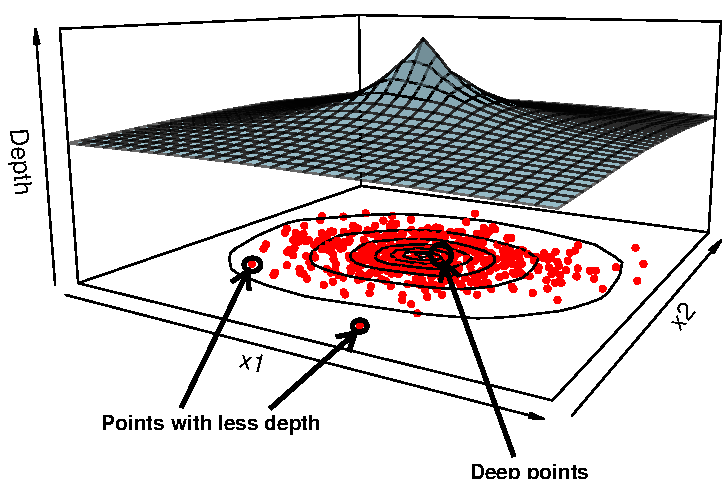
\includegraphics[width=7cm]{Chapter-regression/depthplot_cropped}
	\caption{Depth is a scalar measure of how much inside a point is with respect to a data cloud: 500 points from $\cN_2 ((0,0)^T, \diag (2,1))$}
	\label{fig:depthplot}
\end{figure}

In order to standardizing this notion \cite{liu90} outlined the desirable properties of a statistical depth function:

\vspace{1em}
\noindent\textbf{(P1)} \textit{Affine invariance}: $D(A\bfx + \bfb, \bfA F + \bfb) = D(\bfx, F)$ for any $\bfA\ \in \BR^{p \times p}, \bfb \in \BR^p$. Here $\bfA F + \bfb$ is a slight abuse of notation, and denotes the distribution of $\bfA \bfX + \bfb$ where $\bfX \sim F$;

\noindent\textbf{(P2)} \textit{Maximality at center}: $D(\bftheta, F) = \sup_{\bfx\in \mathbb{R}^p} D(\bfx, F)$ for $F$ having center of symmetry $\bftheta$. This point is called the \textit{deepest point} of the distribution.;

\noindent\textbf{(P3)} \textit{Decreasing from deepest point along any ray}: $D(\bfx; F) \leq D(\bftheta + a(\bfx - \bftheta), F)$;

\noindent\textbf{(P4)} \textit{Vanishing at infinity}: $D(\bfx; F) \rightarrow 0$ as $\|\bfx\| \rightarrow \infty $.

\vspace{1em}
In (P2) the types of symmetry considered can be central symmetry, angular symmetry and halfspace symmetry. Also for multimodal probability distributions, i.e. distributions with multiple local maxima in their probability density functions, properties (P2) and (P3) are actually restrictive towards the formulation of a reasonable depth function that captures the shape of the data cloud. Finally we think affine invariance is an artifact of depth functions being formulated keeping robustness with respect to elliptical distributions in mind, and in most practical cases a location and scale invariance suffices. Furthermore, because of their formulations, technical properties like quasi-concavity, Lipschitz continuity, uniform convergence rise naturally in different definitions of data depth \citep{liu90, zuo00, MoslerChapter13}.

It should be noted here that likelihood is not same as depth. Although in the univariate case many of these are essentially functions of the cumulative distribution function, and indeed for elliptical multivariate distributions depth contours coincide with density contours, unlike depths, likelihood is a local property. It is sensitive to multimodality, does not measure `inlyingness' to a distribution in general and the maximum likelihood point may not be a central point according to any definition of symmetry \citep{serfling2006}.

%A real-valued function measuring the \textit{outlyingness} of a point with respect to the data cloud can be seen as the opposite of what data depth does. Indeed, such functions have been used to define several depth functions, for example simplicial volume depth, projection depth and $L_p$-depth. Let us now formally define such functions as a transformation on any depth function:
%
%\begin{Definition}
%Given a random variable $\bfX$ following a probability distribution $F$, and a depth function $D(.,.)$, we define Htped of a point $\bfx$ as: $\tilde D(\bfx, F) = h(d_\bfx)$ as any function of the data depth $D(\bfx, F) = d_\bfx$ so that $h(d_\bfx)$ is bounded, monotonically decreasing in $d_\bfx$ and $\sup_\bfx \tilde D(\bfx, F) < \infty$.
%\end{Definition}
%
%For a fixed depth function, there are several choices of a corresponding htped. We develop our theory assuming a general htped function, but for the plots and simulations, fix our htped as $\tilde D(\bfx, F) = M_D(F) - D(\bfx, F)$, i.e. simply subtract the depth of a point from the maximum possible depth over all points in sample space.

Some popular measures of data depth available in the literature and extensively used in nonparametric and semiparametric inference are as follows:

\begin{itemize}
\item \textbf{Halfspace depth} (HD: \citep{tukey75}) is defined as the minimum probability of all halfspaces containing a point. In our notations,
%
$$ HD(\bfx, F)  = \inf_{\bfu \in \mathbb{R}^p; \bfu \neq \bf0} P(\bfu^T \bfX \geq \bfu^T \bfx) $$
%
\item \textbf{Mahalanobis depth} (MhD: \cite{LiuPareliusSingh99}) is based on the Mahalanobis distance of $\bfx$ to $\bfmu$ with respect to $\Sigma$: $d_\bfSigma(\bfx, \bfmu) = \sqrt{(\bfx - \bfmu)^T \bfSigma^{-1} (\bfx - \bfmu)}$. It is defined as
%
$$ MhD(\bfX, F) = \frac{1}{1 + d^2_\bfSigma (\bfx, \bfmu)} $$
%

\item \textbf{Projection depth} (PD: \cite{zuo03}) is another depth function based on an outlyingness function. Here that function is
%
$$ O(\bfx, F) = \sup_{\| \bfu \| = 1} \frac{| \bfu^T\bfx - m(\bfu^T\bfX)|}{s(\bfu^T\bfX)} $$
%
where $m$ and $s$ are some univariate measures location and scale, respectively. Given this the depth at $\bfx$ is defined as $PD(\bfx, F) = 1/(1+O(\bfx, F))$.
\end{itemize}

\section{Why is depth not a thing yet?}
Although some articles on data depth are fairly well-cited (e.g. \cite{LiuPareliusSingh99,VardiZhang00}), in general it remains an esoteric, at best intriguing, concept in statistical literature. This is partly due to its nonparametric nature and high computational cost. There have been several approaches for calculating HD. A recent paper \citep{Dyckerhoff16} provides a general algorithm that computes exact HD in $O(n^{p-1}\log n)$ time. PD is generally approximated by taking maximum over a number of random projections: and has high variability for small samples. MhD is easy to calculate since the sample mean and covariance matrix are generally used as estimates of $\bfmu$ and $\bfSigma$, respectively. However this makes it less robust with respect to outliers: defeating the purpose of using data depth in many situations.

A more significant reason though, we believe, is that the concept has not generalized enough since its first inception. There have been attempts at defining depth contours for distributions with nonstandard shapes (multimodal, star-shaped etc.) \citep{PaindaveineJASA2013,Chernozhukov17} as well as using functional depths \citep{NarisettyNair16,Sguera16}. These certainly broaden the domain of application for data depth. However, the scope of using depth, or depth-like quantities, is much larger in statistical inference. It quantifies the proximity of a point in a multivariate space to a probability distribution on the same space. In this spirit, given some hilbert space $\cH$, any such proximity measure $D:\cH \times \tilde \cH \mapsto [0, \infty)$, $\tilde \cH$ being the space of probability measures on $\cH$, can be termed a depth function. Such quantities (or more accurately, decreasing transformations of them, e.g. the outlyingness function of \cite{zuo00}) provide a bridge between point norms and distributional distance measures like the Kullback-Leibler divergence or the Wasserstein metric in appropriate normed spaces. To the best of our knowledge, this generalized notion of point-to-distribution distance/ proximity is absent in the current literature. This thesis is an attempt in leveraging the extra flexibility provided by the above interpretation of data depth functions in diverse inferential scenarios. 

\section{Summary of work}

In \ref{chapter:evalue-chapter}, we consider a general modelling framework in which several parameters need to be estimated from the data. Our objective here is to characterize subsets of the model space based on a pre-defined criterion, and to estimate this characterization in the presence of data. A concrete example for this can be variable selection in linear regression, where the user needs to find out the most parsimonious subset of predictors that do not compromise the quality of model fit. For this purpose we introduce a function called the \textit{statistical evaluation map}, which, while essentially serving the same purpose as depth, are based on much weaker assumptions and take into account the potentially expanding space of parameters. In a transformed space, this evaluates a function of estimated parameters corresponding to a specific subspace with respect to the sampling distribution of parameters from the full parameter space (i.e. the full model). The value of this evaluation function will change based on the specific sample the model estimates are based on, so this has a distribution as well, which depends on the sample size. We name the average evaluation function as the $e$-value of a model: this acts as a quantification of model evidence. Under a very general definition of `good' and `bad' models we demonstrate how these $e$-values can be used to differentiate between these two types. We use resampling to estimate the random distributions we work with: this is essential towards calculating sample version of model $e$-values. As a special case, when data depths are considered as evaluation maps, some further refinement can be achieved in the bifurcation of set of candidate models for the traditional statistical model selection problem. This results in an extremely fast, almost trivial, algorithm to separate out essential predictors in a regression-like setup.

Although depth functions did serve as our motivation for the above work and our initial results were assuming depths in elliptical sampling distributions of parameters, we later found out that a majority of the results hold in a much more generalized setup, and it is enough to explicitly invoke the usage of depths for variable selection only. As demonstrated in \ref{chapter:appli-chapter}, the method of $e$-values leads to valuable insights in several real data situations. In \ref{sec:TwinSection} therein, we expand the scope of $e$-values by considering tail quantiles of evaluation map distributions as $e$-values instead of their means: this leads to improved detection of weak single nucleotide polymorphism signals in behavioral trait analysis of genetic data from families.

\ref{chapter:scatter-chapter} onwards we take a more mainstream approach. Here we introduce a composition of the spatial sign function \citep{LocantoreEtal99} with transformations on functions that are essentially the outlyingness maps of \cite{zuo00}, with a few restrictions for technical convenience. After a brief consideration of its performance in the location problem for elliptical distributions, we define a multivariate rank vector using this. We discuss several aspects of its performance in estimating components of the covariance matrix in the data-generating elliptical distribution: its eigenvectors, eigenvalues and the covariance matrix itself. Several simulation studies and data examples outline the utility of these methods, and we also discuss their implementation in Sufficient Dimension Reduction \citep{AdragniCook09} and functional outlier detection.

\ref{chapter:regression-chapter} discusses another application of the idea of data depth-based inverse ranking, this time in regularized regression. We propose a new class of nonconvex penalty functions in the paradigm of multitask sparse penalized regression using penalties based on data depth. Focusing on a one-step sparse estimator of the coefficient matrix using local linear approximation of the penalty function, we derive its theoretical properties and provide the algorithm for its computation. For orthogonal design and independent responses, the resulting thresholding rule enjoys near-minimax optimal risk performance, similar to the adaptive lasso \citep{Zou06}. A simulation study as well as real data analysis demonstrate its effectiveness compared to some of the present methods that provide sparse solutions in multivariate regression.

%in section e analyzing principal components for multivariate data from its spatial sign covariance matrix (SCM) has been proposed as a computationally simple and robust alternative to normal PCA \citep{LocantoreEtal99}, but it suffers from poor efficiency properties and is actually inadmissible with respect to the maximum likelihood estimator. In chapter \ref{chapter:chap2} we use data depth-based spatial ranks in place of spatial signs to obtain the orthogonally equivariant Depth Covariance Matrix (DCM) and use its eigenvector estimates for PCA. We derive asymptotic properties of the sample DCM and influence functions of its eigenvectors. The shapes of these influence functions indicate robustness of estimated principal components, and good efficiency properties compared to the SCM. Finite sample simulation studies show that principal components of the sample DCM are robust with respect to deviations from normality, as well as are more efficient than the SCM and its affine equivariant version, Tyler's shape matrix. Through two real data examples, we also show the effectiveness of DCM-based PCA in analyzing high-dimensional data and outlier detection, and compare it with other methods of robust PCA.
%
%In chapter \ref{chapter:chap3} we introduce a one-step technique for general regression estimators to provide a solution to the problem of statistical model selection. Under very general assumptions, this method correctly identifies the set of non-zero values in the true coefficient (of length $p$) by comparing only $p + 1$ models. We start by defining our selection criterion for a class of candidate models larger than considered before, and providing population-level results that differentiate between correct and wrong models within this class. After this we provide results for a general bootstrap scheme to estimate the criterion in a sample setup, and discuss its details for linear and linear mixed models. Simulations and a real data example demonstrate the efficacy of our method over existing model selection strategies in terms of detecting the correct set of predictors as well as accurate out-of-sample predictions. At the end we also discuss some immediate applications and possible extensions of this foundational methodology.
%
%We provide an outline of a future project in chapter \ref{chapter:chap4}. Here we propose an iterated reweighted least square algorithm for robust estimation of regression coefficients that uses depths of residuals as weights. Through a simulation study we demonstrate the commendable performance of the algorithm, and then provide a broad sketch of our plans on developing the concept.